%
% This is the LaTeX template file for lecture notes for CS267,
% Applications of Parallel Computing.  When preparing 
% LaTeX notes for this class, please use this template.
%
% To familiarize yourself with this template, the body contains
% some examples of its use.  Look them over.  Then you can
% run LaTeX on this file.  After you have LaTeXed this file then
% you can look over the result either by printing it out with
% dvips or using xdvi.
%

\documentclass[titlepage]{article}


%% \setlength{\oddsidemargin}{-0.25 in}
%% %% \setlength{\evensidemargin}{-0.25 in}
%% \setlength{\topmargi�?n}{-0.6 in}
%% \setlength{\textwidth}{6.5 in}
%% \setlength{\textheight}{8.5 in}
\usepackage[margin=1in]{geometry}
\usepackage{color}
\setlength{\headsep}{0.75 in}
\setlength{\parindent}{0 in}
\setlength{\parskip}{0.1 in}
\usepackage{graphicx}
\usepackage{subfig}
\usepackage{float}
\graphicspath{ {images/} }

\usepackage[compact]{titlesec}

\addtolength{\topmargin}{-.3in}

%
% ADD PACKAGES here:
%

\usepackage{amsmath,amsfonts,graphicx}
\usepackage{tikz}
\usepackage{hyperref}
\hypersetup{
    colorlinks=true,
    linkcolor=teal,
    filecolor=magenta,      
    urlcolor=magenta,
}
\usepackage{color}
\usepackage{enumitem}
\setlist{nolistsep}
 
\urlstyle{same}


\newenvironment{nstabbing}
  {\setlength{\topsep}{-\parskip}%
   \setlength{\partopsep}{0pt}%
   \tabbing}
  {\endtabbing}

%
% The following commands set up the lecnum (lecture number)
% counter and make various numbering schemes work relative
% to the lecture number.
%
\newcounter{lecnum}
\renewcommand{\thepage}{\thelecnum-\arabic{page}}
\renewcommand{\thesection}{\thelecnum.\arabic{section}}
\renewcommand{\theequation}{\thelecnum.\arabic{equation}}
\renewcommand{\thefigure}{\thelecnum.\arabic{figure}}
\renewcommand{\thetable}{\thelecnum.\arabic{table}}

\renewcommand\thesection{\arabic{section}}
\renewcommand\thesubsection{\thesection.\arabic{subsection}}

%
% The following macro is used to generate the header.
%
\newcommand{\lecture}[4]{
   \pagestyle{myheadings}
   \thispagestyle{plain}
   \newpage
   \setcounter{lecnum}{#1}
   \setcounter{page}{1}
   \noindent
   \begin{center}
   \framebox{
      \vbox{\vspace{2mm}
    \hbox to 6.28in { {\bf CMPSCI 311: Introduction to Algorithms
		\hfill Fall 2016} }
       \vspace{6mm}
       \hbox to 6.28in { {\Large \hfill \textbf{Algorithms Final Review}  \hfill} }
       \vspace{4mm}
       %\hbox to 6.28in { \textbf{Name: Gahyun (Susie) Kim} \hfill \textbf{Collaborators}: {} }
       %% \hbox to 6.28in { {\it Lecturer: #3 \hfill Scribes: #4} }
      \vspace{2mm}}
   }
   \end{center}
   \markboth{Homework 2}{Homework 2}

   \vspace*{1mm}
}
%
% Convention for citations is authors' initials followed by the year.
% For example, to cite a paper by Leighton and Maggs you would type
% \cite{LM89}, and to cite a paper by Strassen you would type \cite{S69}.
% (To avoid bibliography problems, for now we redefine the \cite command.)
% Also commands that create a suitable format for the reference list.
\renewcommand{\cite}[1]{[#1]}
\def\beginrefs{\begin{list}%
        {[\arabic{equation}]}{\usecounter{equation}
         \setlength{\leftmargin}{2.0truecm}\setlength{\labelsep}{0.4truecm}%
         \setlength{\labelwidth}{1.6truecm}}}
\def\endrefs{\end{list}}
\def\bibentry#1{\item[\hbox{[#1]}]}

%Use this command for a figure; it puts a figure in wherever you want it.
%usage: \fig{NUMBER}{SPACE-IN-INCHES}{CAPTION}
\newcommand{\fig}[3]{
			\vspace{#2}
			\begin{center}
			Figure \thelecnum.#1:~#3
			\end{center}
	}


\newcommand\numberthis{\addtocounter{equation}{1}\tag{\theequation}}

% Use these for theorems, lemmas, proofs, etc.
\newtheorem{theorem}{Theorem}[lecnum]
\newtheorem{lemma}[theorem]{Lemma}
\newtheorem{proposition}[theorem]{Proposition}
\newtheorem{claim}[theorem]{Claim}
\newtheorem{corollary}[theorem]{Corollary}
\newtheorem{definition}[theorem]{Definition}
\newenvironment{proof}{{\bf Proof:}}{\hfill\rule{2mm}{2mm}}

% **** IF YOU WANT TO DEFINE ADDITIONAL MACROS FOR YOURSELF, PUT THEM HERE:

\newcommand\E{\mathbb{E}}

\begin{document}
%FILL IN THE RIGHT INFO.
%\lecture{**LECTURE-NUMBER**}{**DATE**}{**LECTURER**}{**SCRIBE**}

%\footnotetext{These notes are partially based on those of Nigel Mansell.}

% **** YOUR NOTES GO HERE:

% Some general latex examples and examples making use of the
% macros follow.  
%**** IN GENERAL, BE BRIEF. LONG SCRIBE NOTES, NO MATTER HOW WELL WRITTEN,
%**** ARE NEVER READ BY ANYBODY.


\begin{titlepage}
\vspace{40mm}
\author{Your Best Chingu}
\title{\textbf{CS390MB: \\ Mobile Health Sensing \& Monitoring}}
\maketitle
\end{titlepage}


%********************************************************
%**** SENSOR DATA SMOOTHING & FILTERING
%********************************************************
\section{Sensor Data Smoothing \& Filtering}
\begin{itemize}
\item Sensor data is affected by \textbf{noise} - unexplained variations in data that is uninterpretable. 
\item Goal: Remove noise while retaining important characteristics of signal
\end{itemize}

Noise Removal Techniques can be divided into two classes:
\begin{itemize}
\item Time-domain: intuitive way of approaching problem
\item Frequency-domain: removes noise that is periodic in domain
\end{itemize}


\subsection{Information in Signals}
Two common ways for info to be represented in naturally occurring signals:
\begin{itemize}
\item \textbf{Time domain}: describes when something occurs and what the amplitude
\item \textbf{Frequency}: domain: indirect, measures frequency, phase, and amplitude of periodic motion
\end{itemize}

\subsection{Noisy Sensor Signals}
\begin{figure}[!htb]
  \centering
  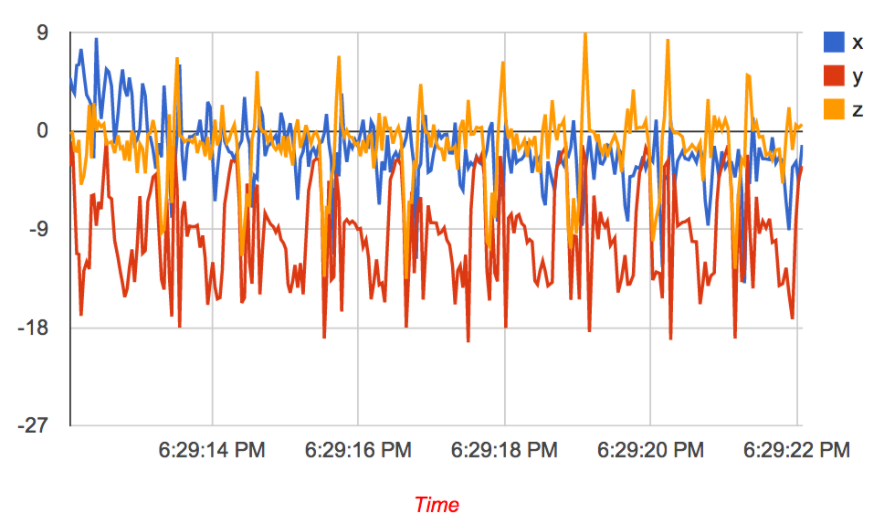
\includegraphics[width=0.7\textwidth]{accelerometer_noise}
  \caption*{Typical Pattern of x,y, and z accelerations while walking with smartphone}
\end{figure}

\textbf{Noise in Accelerometer Data}: categorized into two types:

\textbf{Intrinsic Sensor Noise}
\begin{itemize}
\item Electronic noise from circuitry that is converting motion
\item Mechanical noise of sensor
\end{itemize}

\textbf{External Vibration Noise}
\begin{itemize}
\item Continuous external vibrations induced by earth's movement, nearby vehicles, etc
\item Tiny movements manifest as small changes in accelerometer reading
\item Example: Trying to detect orientation of phone
\subitem Vibrants cause accel. outputs to appear jittery
\subitem Jitters need to be smoothed before applying algorithm to determine screen orientation
\end{itemize}

\newpage

\begin{figure}[!htb]
  \centering

  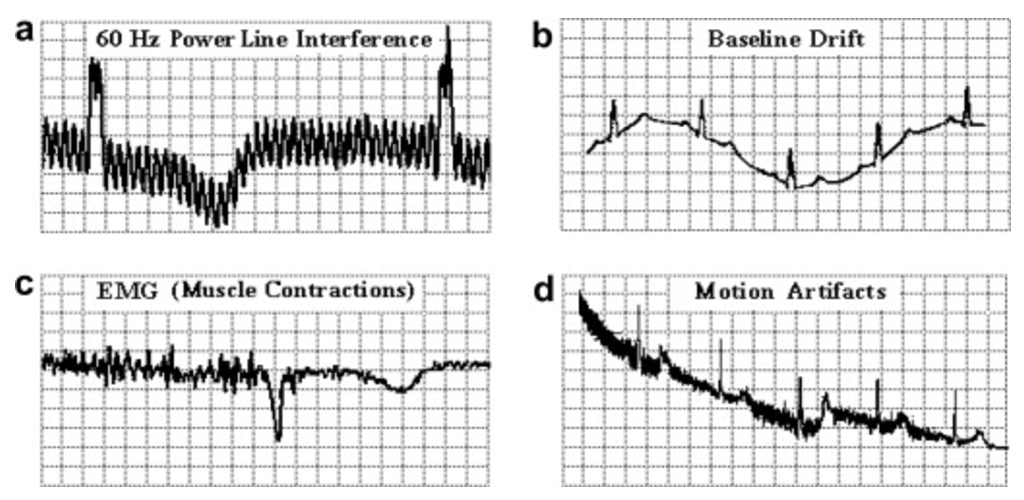
\includegraphics[width=0.8\textwidth]{ecg_noise}
  \caption*{Typical ECG signal with different interference sources}
\end{figure}
\textbf{Noise in Electrocardiogram (ECG) Data}
\begin{itemize}
\item Problem: \underline{power line interference}: 50Hz signal causes electromagnetic interference 
\item Issue is problematic for \underline{low frequency signals} like ECG
\item Other noise: breathing, muscle contractions, body movements, etc
\end{itemize}

\textbf{Noise in Image Data}
\begin{itemize}
\item Noise is often caused by camera
\item Poor illumination conditions, high temperature, electronic noise in circuit
\end{itemize}

\begin{figure}[!htb]
  \centering
  \subfloat[Original Audio Signal]{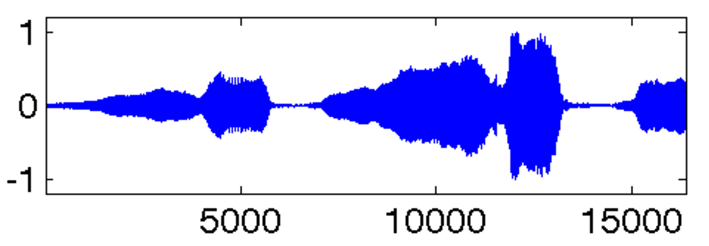
\includegraphics[width=0.3\textwidth]{original_audio}}
  \quad \quad
  \subfloat[Noisy Audio Signal]{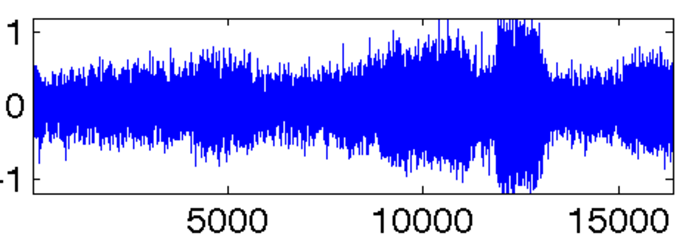
\includegraphics[width=0.3\textwidth]{noisy_audio}}
\end{figure}
\textbf{Noise in Audio Signals}
\begin{itemize}
\item Noise could be due to ambient sound or loud noise nearby such as a construction site
\item Hardware and circuit could add to noise
\end{itemize}

\vspace{2mm}
\begin{figure}[!htb]
  \centering
  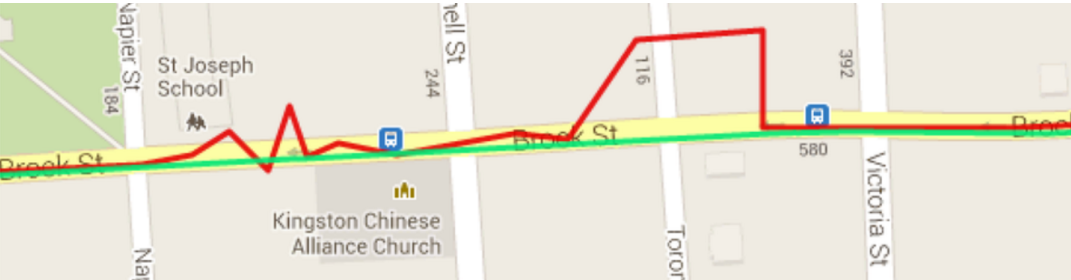
\includegraphics[width=0.55\textwidth]{gps_noise}
  \caption*{Noisy GPS Readings while driving (red), Actual trajectory (green)}
\end{figure}

\vspace{-2mm}
\textbf{Noise in GPS Data}
\begin{itemize}
\item Noise due to clock error, multipath effects due to buildings, weather conditions
\item Raw data coming from GPS receiver has noise that is being smoothed before display
\end{itemize}


\newpage


\subsection{Time-series Smoothing and Filtering}
\textbf{Over-sampling and Averaging}
\begin{itemize}
\item Many sources of noise are random: has roughly equal amounts of positive and negative changes 
\item Noise is uncorrelated in time, has zero mean, and finite variance 
\vspace{1mm}
\item Noise can be reduced by \textbf{oversampling} the sensor and \textbf{averaging} the values
\item Example: 
\subitem Can use a sampling rate of 100 Hz 
\subitem Average every 10 samples readings
\subitem Report average value at 10Hz frequency
\vspace{1mm}
\item If we have $n$ samples of a random noise signal and average them, we reduce noise by a factor of $1/\sqrt{n}$
\end{itemize}

\textbf{Moving Average Smoothing}
\begin{itemize}
\item Replace each sample by average of current sample, sample before, and sample after
\item Let us represent input accelerometer signal as follows: $x = x_1,x_2,...,x_n$ where index is sample number
\item Output of moving average filter:
\begin{align*}
s_1 &= (x_1 + x_2 + x_3) / 3 \\
s_2 &= (x_2 + x_3 + x_4) / 3 \\
s_3 &= (x_3 + x_4 + x_5) / 3 \\ 
 s_{n-2}&=(x_{n-2} + x_{n-1} + x_n) /3
\end{align*}
\item Increasing smoothing window will make signal look cleaner and visually pleasing
\item However, too large a window can smooth out important characteristics of signal
\item Moving Average assumes random noise
\end{itemize}


\textbf{Exponential Smoothing}
\begin{itemize}
\item Effective when noise is time varying
\item Similar to moving average, but assigns exponentially decreasing weights as observations get older
\item Recent observations are given relatively more weight than older observations
\vspace{1mm}
\item smoothing factor $\alpha$:  $0 < \alpha < 1$, 
\item Smoothed output $s_t$: weighted average of current observation $x_t$ and previous smoothed output $s_{t-1}$
\begin{align*}
s_1 &= x_0 \\
s_t &= \alpha x_{t-1} + (1-\alpha )s_{t-1} \\
&= \alpha x_{t-1} + \alpha (1-\alpha)x_{t-2} + (1-\alpha)^2s_{t-2} \\
&= \alpha [x_{t-1} + (1- \alpha)x_{t-2} + (1- \alpha)^2x_{t-3} + (1- \alpha)^3x_{t-4} + ... ] + (1- \alpha)^{t-1}x_0
\end{align*}
\item Larger values of $\alpha$ reduce the level of smoothing
\item $\alpha = 1$ is same as original series (with lag of one time unit)
\end{itemize}
\begin{figure}[!htb]
  \centering
  \subfloat[Signal during walking without smoothing]{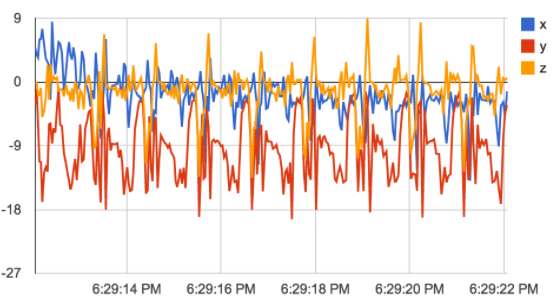
\includegraphics[width=0.35\textwidth]{before_exponential}}
  \quad \quad
  \subfloat[After exponentially weighted smoothing]{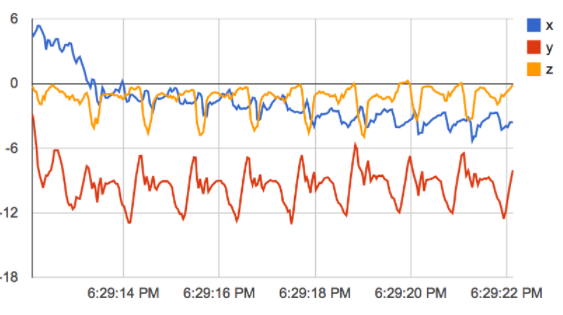
\includegraphics[width=0.35\textwidth]{after_exponential}}
\end{figure}

\newpage
\textbf{Median Filtering}
\begin{itemize}
\item When noise appears like \underline{sudden spikes}, moving average and exponential smoothing are not appropriate
\item Exponential smoothing will average some peaks in data and don't have same amplitude and has lag
\end{itemize}
\begin{figure}[!htb]
  \centering
  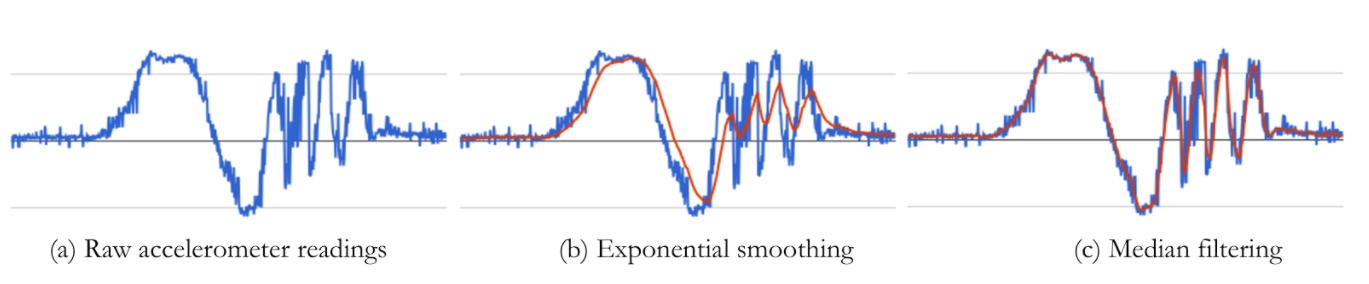
\includegraphics[width=0.9\textwidth]{median_filtering}
  \caption*{Median filtering is better for removing salt-and-pepper noise than exponential smoothing}
\end{figure}
\begin{itemize}
\item Operates over sliding windows like moving average and exponential smoothing
\item Computes median over each window rather than average
\vspace{1mm}
\item If input accelerometer signal is $x = x_1,x_2,...,x_n$, output of median filter is:
\begin{align*}
s_1 &= \text{median}(x_1,x_2,x_3) \\
s_2 &= \text{median}(x_2,x_3,x_4) \\
... \\
s_{n-2} &= \text{median}(x_{n-2},x_{n-1},x_n)
\end{align*}
\end{itemize}


\subsection{Frequency-domain Filtering}
\begin{itemize}
\item Low-pass filter lets low-freq components below threshold through while removing high freq components
\item High-pass filter does reverse and lets high freq components through while removing low freq components
\item Notch filter removes a specific frequency from signal
\end{itemize}

\textbf{ECG Noise Removal}
\begin{figure}[!htb]
  \centering
  \subfloat[ECG signal with baseline wander, powerline interference, and high-freq noise]{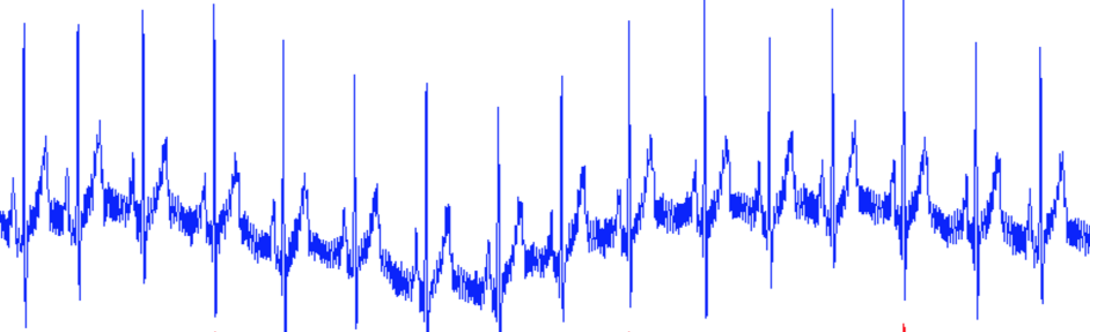
\includegraphics[width=0.4\textwidth]{ecg_wander}}
  \quad \quad
  \subfloat[Filtered ECG Signal]{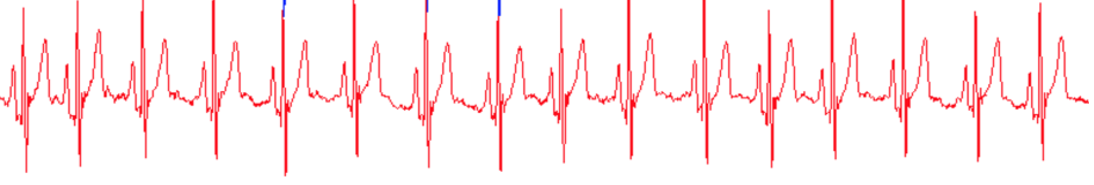
\includegraphics[width=0.4\textwidth]{ecg_filter}}
\end{figure}

\textbf{Baseline Wander}: low-frequency component present in ECG system which causes signal to "wander" off from actual ECG waveform
\begin{itemize}
\item Due to offset voltages in electrodes, periodic breathing, body movement
\item In figure, baseline wander is slowly oscillating waveform with much lower frequency than ECG signal
\item Can be removed by using high-pass filter with cutoff to remove baseline wander
\end{itemize}

\textbf{Powerline Noise}: frequency of alternating current in electrical mains is around 50-60Hz.
\begin{itemize}
\item Can be removed from ECG signal with notch filter at 50/60Hz
\end{itemize}

\textbf{High Frequency Noise}: Pacemakers, phones, other electronics are sources of high frequency noise
\begin{itemize}
\item Removed with low-pass filter
\end{itemize}



\newpage
%******************************************************************
%**DESIGNING PEDOMETER AND CALORIE COUNTER
%******************************************************************
\section{Designing a Pedometer}
Acceleration changes as a result of step and can result in changes along all x, y, and z-axes. \newline
Goal: design an \textit{orientation-independent} algorithm

\subsection{Step Detection Algorithm}
\textbf{Smoothing}
\begin{itemize}
\item Average nearby values to remove noise
\item Increasing smoothing windows creates cleaner signal, but may smooth out steps
\end{itemize}

\begin{figure}[!htb]
  \centering
  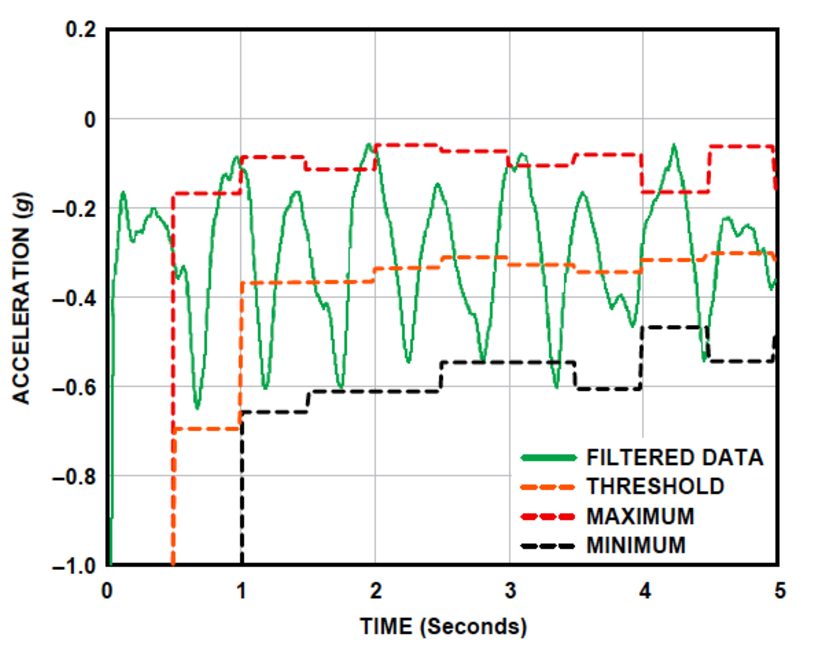
\includegraphics[width=0.5\textwidth]{step_accelerometer}
  \caption*{Filtered data on most active axis}
\end{figure}

\textbf{Dynamic Detection Threshold}
\begin{itemize}
\item No fixed threshold that we can use since threshold depends on orientation of accelerometer
\item Need to use dynamic thresholding scheme to detect a step
\end{itemize}
\begin{enumerate}
\item Keep track of axis along which maximum acceleration occurs
\item Keep track of min and max acceleration levels over a window of samples
\item Average value: (Max + Min)/2 is \textbf{dynamic threshold level} and detects steps for next window sample
\end{enumerate}

\textbf{Step Detection Algorithm}
\begin{itemize}
\item \textbf{Step} is detected if there is a \textbf{negative slope} of acceleration plot when the acceleration curve crosses below the dynamic threshold
\end{itemize}

\textbf{Periodicity}
\begin{itemize}
\item When pedometer vibrates very rapidly or slowly, the step counter will take it as a step
\item Invalid vibrations must be discarded
\end{itemize}
First Approach: Look at time period between any two steps
\vspace{-1mm}
\begin{itemize}
\item Assume people run as fast as five steps per second and walk as slow as one step every two seconds
\item Interval between two valid steps is in range (0.2 to 2.0s)
\item Steps outside time window is discarded 
\end{itemize}
Second Approach: Look for periodic walking pattern 
\vspace{-1mm}
\begin{itemize}
\item Look at time between steps and see if duration repeats (with small variations)
\item Repeated pattern suggests person is walking
\end{itemize}



\newpage
%******************************************************************
%**ACTIVITY RECOGNITION W/ INERTIAL SENSORS
%******************************************************************
\section{Activity Recognition using Inertial Sensors}

\subsection{Detection vs. Classification}
\begin{itemize}
\item With activity recognition, we assume we don't know distinguishing characteristics of each activity
\item Provide training data: sample datasets of each class  
\item Provide features: large set of possible characteristics of data that may be important
\item Let automated algorithm identify what features are most useful to distinguish between classes
\end{itemize}

\subsection{Labeled Data Collection}
\begin{itemize}
\item Labels: ground truth corresponding to raw data must be available
\item Training data is used to develop classification algorithm
\item Carrying phone in different orientations will help algorithm to be less sensitive to orientation variations
\end{itemize}

\subsection{Visualizing Common Activities}
\begin{figure}[!htb]
  \centering
  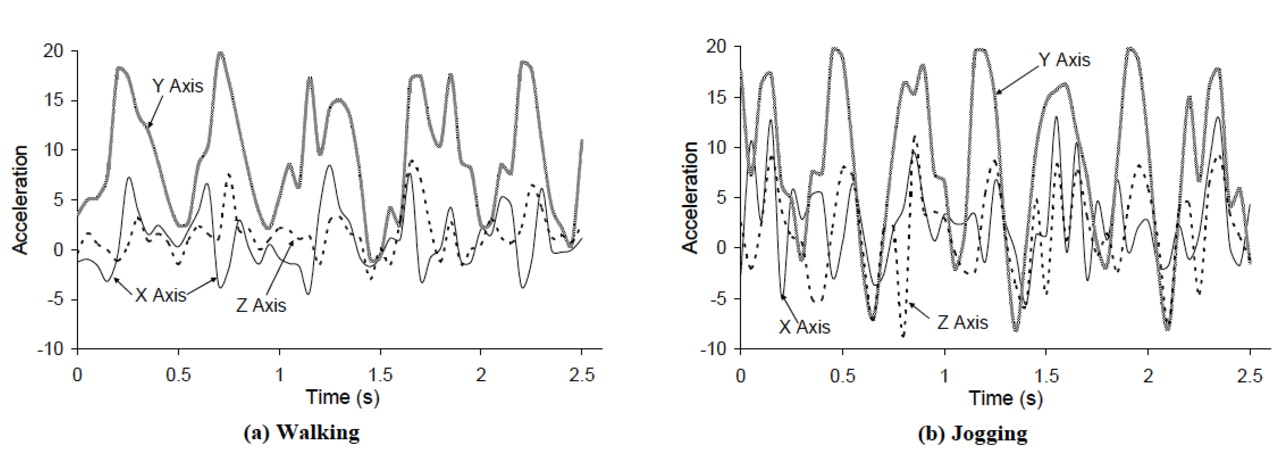
\includegraphics[width=0.85\textwidth]{walking_jogging}
  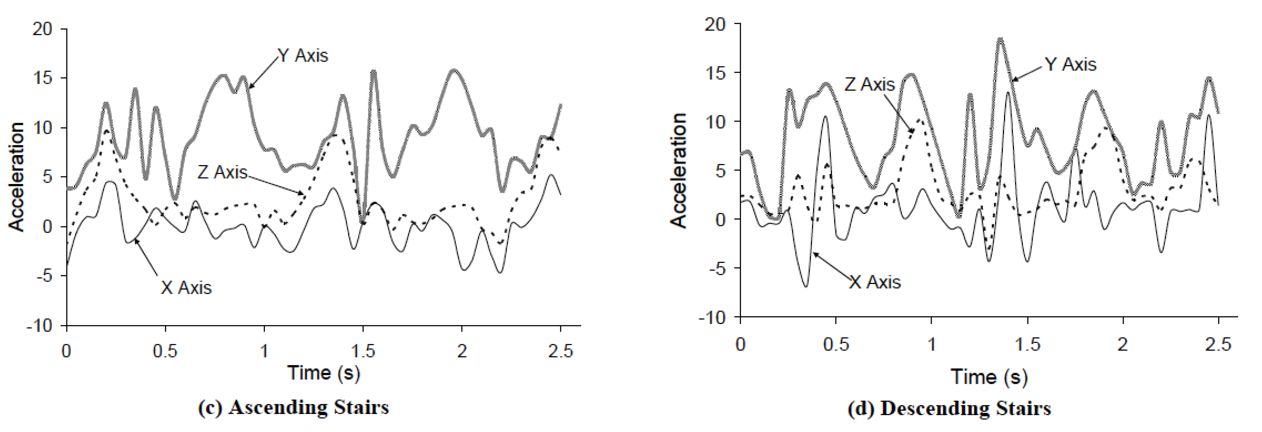
\includegraphics[width=0.85\textwidth]{ascending_descending}
  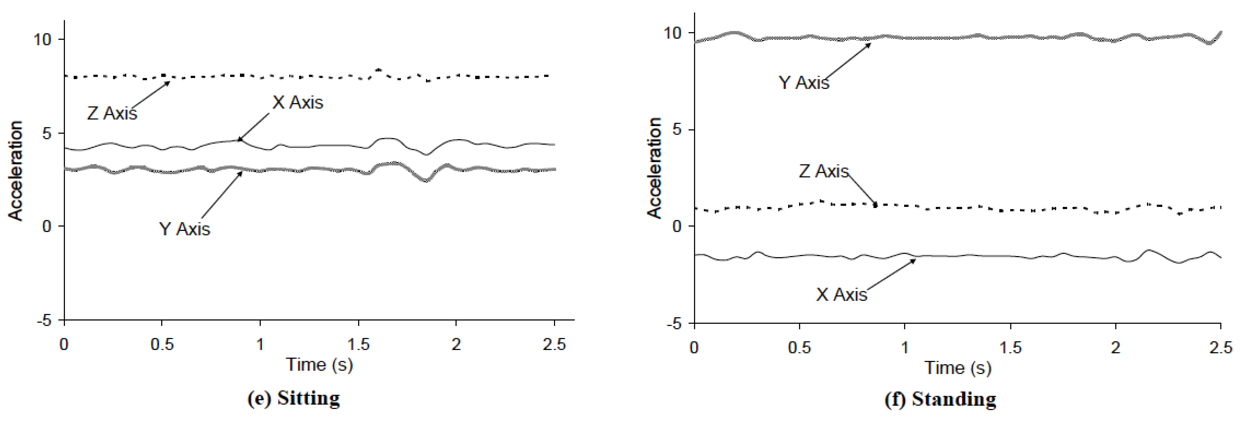
\includegraphics[width=0.85\textwidth]{sitting_standing}
\end{figure}

\newpage

\subsection{Feature Generation \& Data Transformation}
\begin{itemize}
\item Distinguishing features: frequency, frequency changes
\item Useful to divide features into two classes: a) time domain features b) frequency domain features
\end{itemize}
\begin{center}
\begin{tabular}{ c|c }		
  Time Domain Features & Frequency Domain Features  \\
   \hline 
  Mean, Median, Variance, Standard Deviation  & Dominant frequency, Signal Energy \\
  Min, Max, Range, Zero-crossings, Angle, Angular velocity 
\end{tabular}
\end{center}

\subsection{Decision Tree Classifier}
\begin{figure}[!htb]
  \centering
  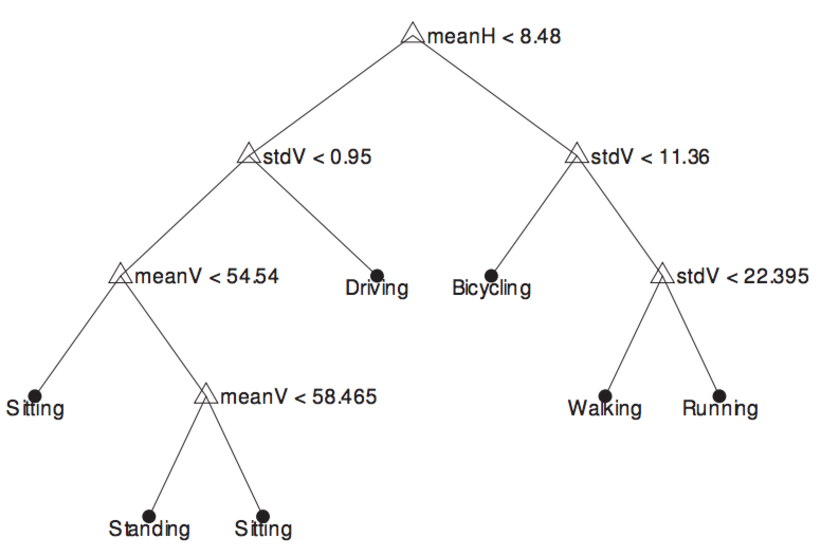
\includegraphics[width=0.6\textwidth]{decision_tree}
\end{figure}

\textbf{Building Decision Tree}
\begin{itemize}
\item At each node of tree, choose attribute of data that most effectively splits set of samples into subsets enriched in one class or other
\item Splitting criterion: \textbf{information gain} - metric for describing how much separation is achieved after split compared to before
\end{itemize}

\textbf{Entropy}
\begin{itemize}
\item A way to measure impurity (0 = minimum impurity, 1 = maximum impurity)
\item Let $p_i$ be probability of class $i$ - compute as proportion of class $i$ in set
\[ \text{Entropy} = \sum_{i} -p_i \log_2{p_i} \]
\end{itemize}

\textbf{Information Gain}
\begin{itemize}
\item Tells us how important a given attribute of the feature vectors is
\[ \text{Information Gain} = \text{entropy(parent)} - \text{[\underline{weighted} average entropy (children)]} \]
\end{itemize}

\textbf{Pseudocode}
\begin{enumerate}
\item For each attribute $a$, find normalized information gain from splitting on $a$
\item Let $a\_best$ be attribute with highest normalized information gain
\item Create decision node that splits on $a\_best$
\item Recurse on sublists obtained by splitting on $a\_best$ and add nodes as children of node
\end{enumerate}



\newpage
%******************************************************************
%**EVALUATING CLASSIFIER PERFORMANCE
%******************************************************************
\section{Evaluating Classifier Performance}
\subsection{Cross Validation}
\textbf{Holdout Method}
\begin{itemize}
\item Data set is separated into two sets: a) training set b) testing set
\subitem common rule: 70\% of dataset for training and 30\% for testing
\item Dividing data into subsets is done randomly to guarantee no systematic error
\vspace{1.5mm}
\item Classifier is learnt using training set only 
\subitem predicts output values for data in testing set
\item Errors are accumulated before to give mean absolute test set error
\end{itemize}

\vspace{2mm}
\textbf{N-fold Cross Validation}
\begin{itemize}
\item Data set is divided into $n$ subsets and holdout method is repeated $n$ times
\item Each time, one of $n$ subsets is used as test and other $n-1$ subsets form training set
\item Average error across all $n$ trials is computed 
\vspace{1.5mm}
\item Advantage: matters less how data gets divided, more robust
\item Disadvantage: training algorithm is rerun $n$ times 
\end{itemize}

\textbf{Overfitting}: phenomenon of relying on patterns that are strong only in training data

\vspace{2mm}
\subsection{Confusion Matrix: Performance Measures}
\begin{itemize}
\item Rows correspond to known class of data
\item Columns correspond to predictions made by model
\item Diagonal elements show number of correct classifications made for each class
\item Off-diagonal elements show errors made
\end{itemize}

\vspace{2mm}
$TP$ and $FP$ are numbers of true positive and false positive predictions for considered class.

\textbf{Accuracy}: overall correctness of model
\vspace{-1mm}
\begin{itemize}
\item Sum of correct classifications divided by total number of classifications
\end{itemize}


\textbf{Precision}: measure of accuracy provided that a specific class has been predicted (cell / sum of column)
\[ \text{Precision} = \frac{TP}{TP + FP} \]

\textbf{Recall}: measure of ability of model to select instances of a certain class from a data set (cell / sum of row)
\[ \text{Recall} = \frac{TP}{TP + FN} \]

\textbf{F-measure}: weighted average of precision and recall (best at 1, worst at 0)
\[ \text{F} = \frac{2 \times \text{Precision} \times \text{Recall}}{\text{Precision} + \text{Recall}} \]


\newpage
%******************************************************************
%**QUANTIFIED SELF & PERSONAL DATA ANALYTICS
%******************************************************************
\section{Quantified Self \& Personal Data Analytics}
\subsection{Quantified Self Movement}
\textbf{Quantified self} is a grassroots movement where people are measuring, logging, and sharing metrics related to their physical and mental health.


\subsection{Obtaining Data About Yourself}
\begin{itemize}
\item Logging data from digital traces (Fitbit, Airline sites, Outlook, etc)
\item Process is not completely monitored (yet)
\end{itemize}

\subsection{Analyzing Lifelog Data for Useful Insights}
\textbf{Visualizing Trends in Data}
\begin{itemize}
\item Charting and plotting trends in each variable 
\end{itemize}

\textbf{Mining Patterns in Data}
\begin{itemize}
\item Association rule mining: useful when you have sequences of labeled data
\subitem Ex: data about food locations visited, attentiveness in class, productivity level, etc
\item Use association rule mining to discover association between food habits and other indicators
\end{itemize}

\textbf{Identifying Predictors}
\begin{itemize}
\item Want to identify predictors for a behavior or variable
\item Example: record weight gain data with checkins for \#visits to coffee shop, \#visits to Chipotle, etc
\item Linear regression: assumes form for relationship between predictors $X_i$ and response variable $y$
\subitem $\beta$ represents weight associated with specific predictor
\[y=\beta_0+\beta_1X_1 + \beta_2X_2 + \beta_3X_3 + \alpha \]
\item After computing coefficients, next Q: how well have we captured trends present in weight gain?
\subitem There may be some other variable affecting weight gain
\vspace{1mm}
\item Look at residual error after fitting and see if there is any pattern in residual error
\subitem If there is a pattern, there is a trend we did not capture using set of predictor variables
\subitem Or relationship between weight and predictive variables is not linear
\vspace{2mm}
\item Next step: figuring out what predictors matter
\item Need a hypothesis test for statistical significance
\vspace{1mm}
\subitem Measure: $p$-value
\vspace{1mm}
\subsubitem Low $p$-value $< 0.05$ means variable is highly predictive
\subsubitem High $p$-value means not useful
\end{itemize}

\textbf{Eliciting Change in Behavior}
\begin{itemize}
\item Goal of self-tracking: fixing a problem and discovering patterns and roots of problem
\end{itemize}

Experimental Design: A = baseline, B = treatment
\begin{itemize}
\item \textbf{AB} : simplest and weakest of all in capturing causality
\item \textbf{ABA}: captures changes in $Y$ before and after treatment
\subitem Helps conclude if treatment works and how long effects last
\item \textbf{ABAB}: useful to capture intensity of treatment is associated with intensity of outcome
\subitem Can compare changes in both treatment phases
\subitem In either treatment phases, can replace one with placebo
\end{itemize}




%******************************************************************
%**VOICE-BASED HEALTH ANALYTICS
%******************************************************************
\section{Voice-based Health Analytics}
\subsection{Voice Analysis Library: Feature Set}
\textbf{Mel-frequency Spectral Coefficients (MFCC)}
\begin{itemize}
\item Extracts features closest to human perception of voice
\item Relates perceived frequency of a pure tone to its actual measured frequency
\item Log of Mel filterbank: human hearing - we don't hear loudness on a linear scale
\subitem To double perceived volume of sound, we need to put 8 times as much energy into it
\end{itemize}

\textbf{Other Audio Features}
\begin{itemize}
\item \textbf{Pitch}: describes how listener perceives a sound
\subitem Sudden increase in pitch $\rightarrow$ high activation, anger
\subitem Low variance of pitch $\rightarrow$ low energy, sadness
\vspace{1.5mm}
\item \textbf{Intensity}: reflects effort to produce speech
\subitem Rapid rise of energy $\rightarrow$ angry utterance
\subitem Low intensity $\rightarrow$ sad speech
\vspace{1.5mm}
\item \textbf{Temporal Aspects}: describes speech rate and voice activity (pauses)
\subitem Can reflect emotions
\vspace{1.5mm}
\item \textbf{Voice Quality}: emotions influence voice quality of utternaces
\subitem Sharp/jagged vs soft
\subitem Glottal waveforms are useful
\subitem Sudden change in air flow produces high frequency
\vspace{1.5mm}
\item \textbf{Spectogram}: describes energy distribution across frequency bands
\subitem Certain frequency may be speaker dependent
\subitem Used to reflect emotions
\vspace{1.5mm}
\item \textbf{Other Statistical Measures}: can help represent all possible dynamics affected by emotions
\end{itemize}


\subsection{Voice Analysis Library: Classification}
\textbf{Speech Processing}
\begin{itemize}
\item Human speech can be broken into phenomes 
\item Challenge in speech recognition: recognizing sequence of phenomes as particular word
\item Speech recognizers use a HIdden Markov Model (HMM)
\end{itemize}

\textbf{Diagnosis of Mental Illness}
\begin{itemize}
\item Aspects of speech help describe patient's state of mind under domains of behavior, cognition, etc.
\item Depressed patients express slow responses, monotonic phrases, and poor articulation
\item Agitated behavior includes expansive gesturing, pacing
\item Gaussian Mixture Model: clustering approach for classifying audio features
\end{itemize}


\subsection{Monitoring Affect with a Mobile Phone}
\begin{itemize}
\item Monitoring stress in everyday lives: phones can monitor stress and inform ways to de-stress
\item Monitoring social interactions (or lack of it)
\end{itemize}


\newpage
%******************************************************************
%**PHYSIOLOGICAL SENSING
%******************************************************************
\section{Physiological Sensing}
\subsection{Electrocardiogram (ECG)}
\textbf{ECG}: recording of electrical activity of heart
\begin{itemize}
\item Each heartbeat: electrical signal spreads from top to bottom of heart
\item Can measure heart's electrical signals by:
\subitem Placing two electrodes at different points on chest 
\subitem Measuring electrical activity between electrodes
\vspace{2mm}
\end{itemize}
\vspace{-1.5mm}
ECG can show:
\vspace{-1.5mm}
\begin{itemize}
\item How fast heart is beating
\item Rhythm of heartbeat (steady vs irregular)
\item Strength and timing of electrical singals 
\end{itemize}

\textbf{Detecting Peaks and Troughs in ECG Waveform}
\begin{itemize}
\item Can use peak detection for step detector
\item Look for change in slope and sequence info to label appropriate peaks
\end{itemize}

\textbf{Extracting ECG Features}
\begin{itemize}
\item Once we get 5 or 6 peaks and troughs, timing differences between each is useful for classification
\item RR interval corresponds to time between two successive heartbeats
\item Computing heartrate: $HR = 60 / RR$
\end{itemize}

\vspace{2mm}
\subsection{Photoplethysmography (PPG)}
\textbf{PPG}: non-invasive technique for measuring blood volume changes in vessels close to skin
\begin{itemize}
\item Place finger over camera with flash
\item Camera records light absorbed by finger tissue
\item Each frame is processed by splitting every pixel into RBH components
\item Components are processed to extract HR and breathing rate
\end{itemize}

\textbf{Extracting Heart Rate from PPG}
\begin{itemize}
\item Changes in arterial blood volume correspond to heart rate
\item When blood retracts, more light passes through tissue
\vspace{2mm}
\item Green intensity average in PPG signal forms peaks corresponding to cardiac pulse
\item Peak: highest average of green values in fixed window size
\item After peak detection: compute time difference between consecutive peaks
\item Time difference = RR interval, $HR = 60/RR$
\end{itemize}

\textbf{Extracting Breathing Rate from PPG}
\begin{itemize}
\item Respiratory Sinus Arrhythmia (RSA): naturally occurring variation in heart rate that occurs in breathing cycle
\item Herat rate increases during inspiration and decreases during expiration
\item We look for frequency of changes in heart rate
\item Use FFT to convert from time to frequency domain and take dominant frequency from FFT
\end{itemize}

\newpage

\subsection{Electrodermal Activity (EDA)}
\textbf{EDA}: measures electrical chnages at skin surface that arise when skin receives innervating signals from brain
\begin{itemize}
\item When people experience emotional arousal, increased cognitive workload or physical exertion:
\subitem Brain sends signals to skin to increase level of sweating 
\vspace{1mm}
\item EDA results from sympathetic neuronal activity - neural response cannot be controlled consciously 
\item Used to examine implicit emotional responses and for lie detection
\end{itemize}

\textbf{EDA Features}: Two main components:
\begin{itemize}
\item Skin Conductance Level (SCL): slower acting components: 
\item Skin Conductance Response (SCR): faster changing components 
\vspace{1mm}
\subitem Example: if startled, SCR changes in seconds while SCL changes over minutes
\end{itemize}

\begin{figure}[!htb]
  \centering
  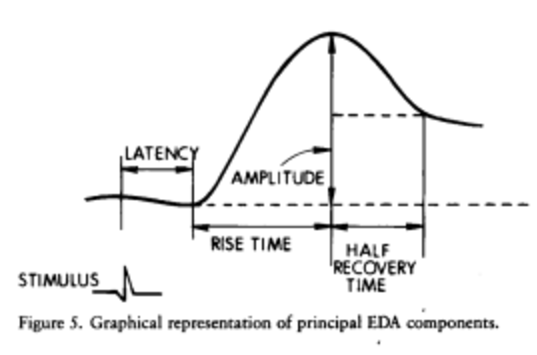
\includegraphics[width=0.5\textwidth]{scr}
  \caption*{Typical SCR}
\end{figure}

SCR can be sub-divided into features useful for classification

\begin{itemize}
\item \textbf{Latency}: amount of time between stimulus and rise of wave
\item \textbf{Rise time}: time for skin conductance to shoot up to peak
\item \textbf{Amplitude}: height of the SCR
\item \textbf{Half recovery time}: amount of time it takes for wave to fall back to half its amplitude
\end{itemize}

\vspace{1mm}
SCL is background signal in absence of SCR
\begin{itemize}
\item Select small window of EDA samples with no SCR
\item SCL level is average value of EDA
\end{itemize}

\newpage
%******************************************************************
%**GPS CLUSTERING AND ANALYTICS
%******************************************************************
\section{GPS Clustering \& Analytics}
\subsection{Clustering Location Data}
\begin{itemize}
\item \textbf{Noise}: GPS error depends on numbers factors: satellites, tall buildings, indoor/outdoor
\item \textbf{Meaningful Clusters}: identifying which GPS coordinates correspond to meaningful clusters
\item \textbf{Semantic Location}: converting clusters to places (home, work, coffee shop)
\end{itemize}

\subsection{GPS Clustering}
\textbf{Phase I: Pre-processing}: removing noise and outliers
\begin{enumerate}
\item Remove low density points
\item Remove points with movement 
\item Reduce data for stationary locations
\end{enumerate}

\textbf{Phase II: Clustering}

\textbf{K-means}: key parameter is $k$, number of clusters

Given k, the k-means algorithm consists of iterative algorithm with 4 steps:
\begin{itemize}
\item Select $k$ initial centroids at random from points
\item \textbf{repeat}
\subitem Assign each object to cluster with nearest centroid (in terms of distance)
\subitem Re-compute each centroid as mean of objects assigned to it
\item \textbf{until} centroids do not change
\end{itemize}

Simple and effective, but has \textbf{limitations}
\begin{itemize}
\item \textbf{Differing sizes}: K-means assumes that cluster are roughly similarly sized
\item \textbf{Differing density}: K-means relies on centroid of points to separate into clusters
\end{itemize}
\begin{figure}[!htb]
  \centering
  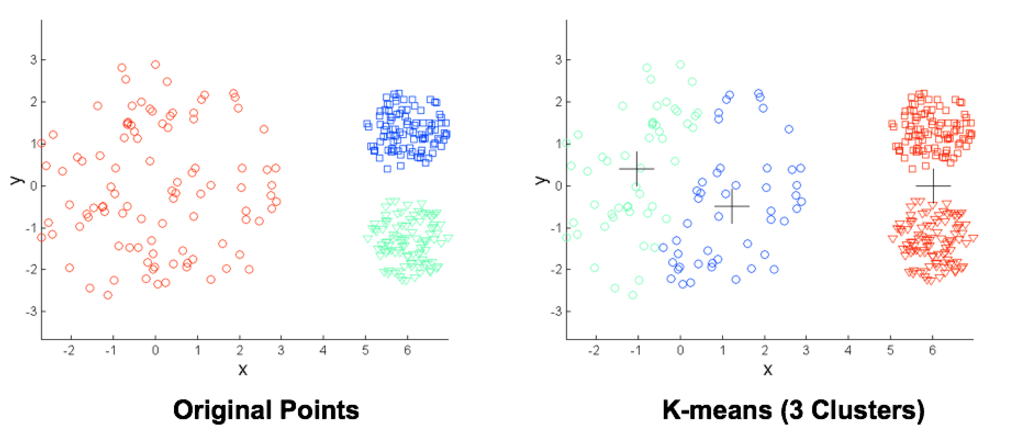
\includegraphics[width=0.55\textwidth]{differing_sizes}
\end{figure}
\vspace{-2mm}
\begin{itemize}
\item \textbf{Non-globular shapes}: K-means cannot deal with irregular and skewed shapes
\end{itemize}
\begin{figure}[!htb]
  \centering
  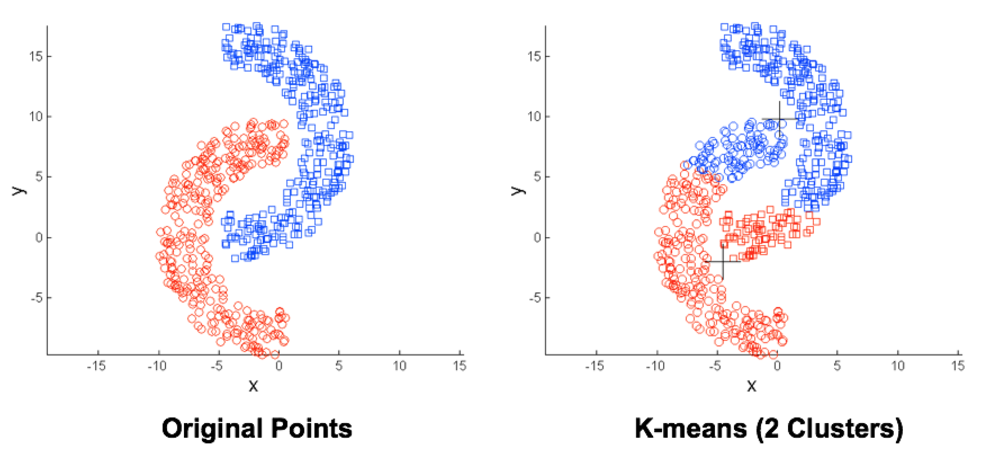
\includegraphics[width=0.55\textwidth]{non-globular}
\end{figure}

\newpage

\textbf{DBSCAN}: assumes cluster is a connected regions where points are relatively dense

\vspace{-2mm}
Requires two parameters: a) $\epsilon$ (eps) b) minPts

Given parameters, points can be separated into three classes:
\begin{itemize}
\item Point is \textbf{core point} if it has more than minPts within $\epsilon$ 
\item \textbf{Border point} has fewer than minPts within $\epsilon$ but is in neighborhood of core point
\item \textbf{Noise point} any point that is not a core point or border point
\end{itemize}


\begin{figure}[!htb]
  \centering
  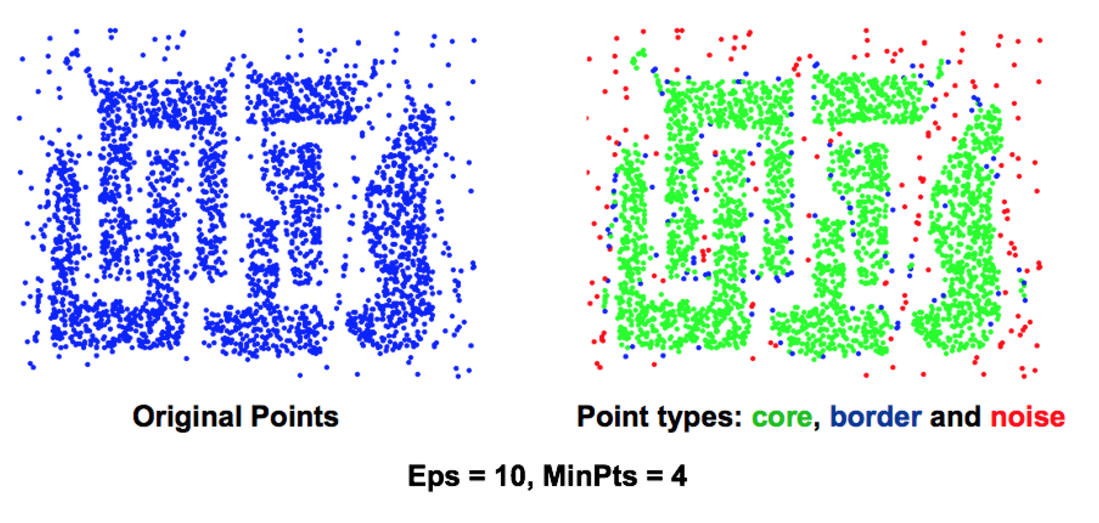
\includegraphics[width=0.7\textwidth]{dbscan}
\end{figure}

\vspace{-2mm}
Once points are divided, DBScan algorithm:
\begin{itemize}
\item Removes all noise points
\item Performs clustering on remaining points in iterative manner
\end{itemize}

\textbf{Pseudocode}
\vspace{-7mm}
\begin{tabbing}
\hspace*{.25in} \= \hspace*{.25in} \= \hspace*{.25in} \= \hspace*{.25in} \= \hspace*{.25in}\= \hspace*{.25in} \=\kill\> \\
\>DBSCAN(D, eps, MinPts)  \\
\>\> C = 0 \\
\>\> \textbf{for} each point P in dataset D \\
\>\>\> \textbf{if} P is visited \\
\>\>\>\> continue next point \\
\>\>\> mark P as visited \\
\>\>\> NeighborPts = regionQuery(P, eps) \\
\>\>\> \textbf{if} sizeof(NeighborPts) $<$ minPts \\
\>\>\>\> mark P as NOISE \\
\>\>\> \textbf{else} \\
\>\>\>\> C = next cluster \\
\>\>\>\> expandCluster(P, NeighborPts, C, eps, MinPts) \\ \\
\> expandCluster(P, NeighborPts, C, eps, MinPts) \\
\>\> add P to cluster C \\
\>\> \textbf{for} each point P' in NeighborPts \\
\>\>\> \textbf{if} P' is not visited \\
\>\>\>\> mark P' as visited \\
\>\>\>\> NeighborPts' = regionQuery(P', eps) \\
\>\>\>\> \textbf{if} sizeof(NeighborPts') $\geq$ MinPts \\
\>\>\>\>\>  NeighborPts = NeighborPts $\cup$ NeighborPts' \\
\>\>\> \textbf{if} P' is not yet a member of any cluster \\
\>\>\>\> add P' to cluster C \\ \\
\> regionQuery(P, eps) \\
\>\> return all points within P's eps-neighborhood (including P) 
\end{tabbing}


\textbf{Mean Shift}: considers feature space as probability density function
\begin{itemize}
\item Does not require prior knowledge of number of clusters and does not constrain cluster shape
\subitem Ideal for handling clusters of arbitrary shape and number
\vspace{1mm}
\item Places a \underline{kernel} on each point in data set
\subitem kernel: a weighting function
\vspace{1mm}
\item Adding all of individual kernels up generates a probability surface
\item Primarily a mode finding algorithm - number of clusters is obtained by number of modes
\end{itemize}

\textbf{High Level Intuition}:
\begin{enumerate}
\item Fix window around each data point
\item Compute mean of data within window
\item Shift window to mean and repeat till convergence
\end{enumerate}

\begin{figure}[!htb]
  \centering
  \subfloat[KDE surface plot]{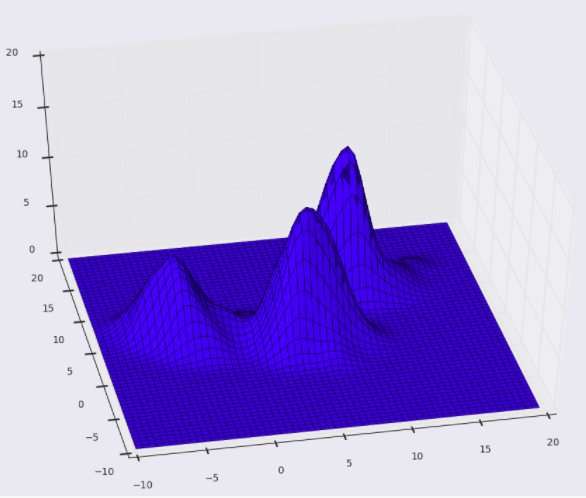
\includegraphics[width=0.3\textwidth]{surface_plot}}
  \quad \quad
  \subfloat[KDE contour plot]{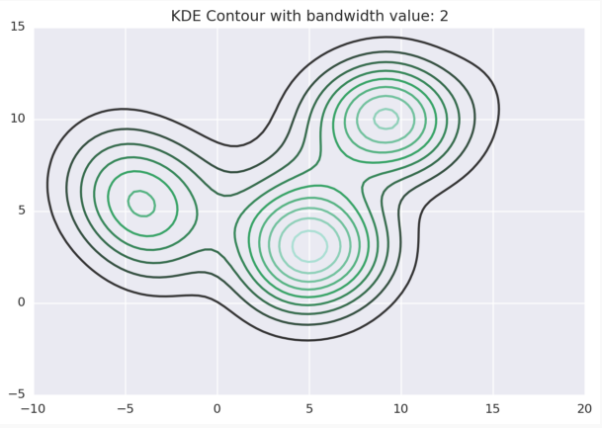
\includegraphics[width=0.38\textwidth]{contour_plot}}
\end{figure}

\vspace{6mm}
\textbf{Phase III: Clusters to Semantic Locations}
\begin{itemize}
\item Can use reverse geo-coding on cluster centroids
\item Going from GPS coordinates of centroid to name of place
\end{itemize}










% ***********************************

\end{document}





